%==============================================================
%  EE201 -- Circuit Theory I
%  Lecture 6 : Dependent Sources and the Ideal Transformer -- slides
%  M. Mert Ankaralı, METU EEE
%
%  Compile:  ./build.sh      (or: pdflatex EE201_Lecture_6_slides.tex, twice)
%  Same colour code as the handout:
%      charge = purple, current = blue, voltage = orange, power = green
%==============================================================
\documentclass[11pt,aspectratio=169]{beamer}

\usepackage[T1]{fontenc}
\usepackage[utf8]{inputenc}
\usepackage[english]{babel}
\usepackage{lmodern}
\usepackage{amsmath,amssymb}
\usepackage{booktabs}
\usepackage{array}
\usepackage{colortbl}
\usepackage{tikz}
\usepackage[american,siunitx]{circuitikz}
\usetikzlibrary{arrows.meta,positioning,calc,decorations.pathreplacing,decorations.pathmorphing,decorations.markings}
\usetikzlibrary{overlay-beamer-styles}

%-------------------- plain METU-flavoured theme --------------
\usetheme{default}
\usecolortheme{default}
\useinnertheme{rectangles}
\setbeamertemplate{navigation symbols}{}
\setbeamertemplate{itemize items}[square]
\setbeamerfont{frametitle}{size=\large,series=\bfseries}
\setbeamerfont{title}{size=\LARGE,series=\bfseries}

\definecolor{metured}{RGB}{155,27,48}
\definecolor{metugray}{RGB}{88,89,91}
\definecolor{metulight}{RGB}{243,240,241}
\definecolor{ccur}{RGB}{0,102,170}
\definecolor{cvolt}{RGB}{214,120,0}
\definecolor{cpow}{RGB}{23,128,74}
\definecolor{ccharge}{RGB}{124,60,160}
\definecolor{cflux}{RGB}{0,138,138}
\definecolor{copper}{RGB}{184,98,30}

\setbeamercolor{structure}{fg=metured}
\setbeamercolor{frametitle}{fg=metured,bg=}
\setbeamercolor{title}{fg=metured}
\setbeamercolor{normal text}{fg=black!88}
\setbeamercolor{block title}{fg=white,bg=metured}
\setbeamercolor{block body}{bg=metulight}
\setbeamercolor{alerted text}{fg=metured}

\setbeamertemplate{frametitle}{%
  \vspace{0.55em}%
  \usebeamerfont{frametitle}\usebeamercolor[fg]{frametitle}\insertframetitle\par
  \vspace{-0.2em}{\color{metured}\rule{\textwidth}{1pt}}\par\vspace{-0.2em}}

\setbeamertemplate{footline}{%
  \hbox{\begin{beamercolorbox}[wd=\paperwidth,ht=2.4ex,dp=1.4ex,leftskip=1.2em,rightskip=1.2em]{}%
  \tiny\color{metugray}\coursecode\ \textbar\ Lecture 6: Dependent Sources and the Ideal Transformer
  \hfill \insertframenumber/\inserttotalframenumber
  \end{beamercolorbox}}}

%-------------------- macros ----------------------------------
\newcommand{\coursecode}{EE201}
\newcommand{\term}{Fall 2026--2027}
\newcommand{\Icol}[1]{\textcolor{ccur}{#1}}
\newcommand{\Vcol}[1]{\textcolor{cvolt}{#1}}
\newcommand{\Pcol}[1]{\textcolor{cpow}{#1}}
\newcommand{\Qcol}[1]{\textcolor{ccharge}{#1}}
\newcommand{\Fcol}[1]{\textcolor{cflux}{#1}}
\newcommand{\uni}[1]{\,\mathrm{#1}}
\newcommand{\A}{\uni{A}} \newcommand{\V}{\uni{V}}
\newcommand{\W}{\uni{W}} \newcommand{\J}{\uni{J}}
\newcommand{\Cb}{\uni{C}} \newcommand{\s}{\uni{s}}
\newcommand{\Wb}{\uni{Wb}} \newcommand{\Hy}{\uni{H}}
\newcommand{\Sie}{\uni{S}}

\ctikzset{bipoles/length=0.9cm, label/align=straight,
          bipoles/vsourceam/height=0.85, bipoles/vsourceam/width=0.85}
\tikzset{
  curarr/.style={-{Stealth[length=2.6mm]}, ccur, very thick},
  blk/.style={draw=metugray, fill=metulight, rounded corners=2pt,
              minimum height=1.25cm, text width=2.45cm, align=center, font=\scriptsize},
  flowarr/.style={-{Stealth[length=3mm]}, metured, very thick},
  thru/.style={-{Stealth[length=2.2mm]}, ccur, very thick},
  acr/.style={{Stealth[length=2mm]}-{Stealth[length=2mm]}, cvolt, very thick},
  pan/.style={draw=gray!35, fill=metulight, rounded corners=3pt,
              minimum width=3.0cm, minimum height=2.3cm},
  pcap/.style={font=\scriptsize\bfseries, text=metured},
  pol/.style={font=\small, text=cvolt},
  iar/.style={-{Stealth[length=2.4mm]}, ccur, very thick},
  gnode/.style={circle, fill=metured, inner sep=0pt, minimum size=4.2pt},
  glab/.style={font=\footnotesize, text=metured},
  surf/.style={draw=cpow, very thick, dashed, rounded corners=6pt},
  gbr/.style={metugray, thick, postaction={decorate, decoration={markings,
      mark=at position 0.58 with {\arrow{Stealth[length=2.4mm]}}}}},
  vax/.style={-{Stealth[length=2mm]}, gray!70},
  crv/.style={metured, very thick},
  ttl/.style={font=\scriptsize\bfseries, text=metugray},
  capn/.style={font=\scriptsize, text=metugray, align=center},
  ampbox/.style={draw=metured!70, thick, dashed, rounded corners=5pt},
  dotm/.style={circle, fill=black, inner sep=0pt, minimum size=4.2pt},
  core/.style={line width=1.1pt, metugray},
  hal/.style={draw=metured!45, line width=7pt, opacity=0.35, line cap=round},
}

\newcommand{\ohm}{\,\Omega}
\newcommand{\Req}{R_{\mathrm{eq}}}
\newcommand{\kohm}{\,\mathrm{k}\Omega}
\newcommand{\xfmr}[2]{%
  \begin{scope}[xshift=#1 cm]
    \ctikzset{bipoles/length=1.35cm}
    \draw (0,0) to[L] (0,#2);
    \draw (1.6,#2) to[L] (1.6,0);
    \draw[core] (0.72,-0.05) -- (0.72,#2+0.05);
    \draw[core] (0.88,-0.05) -- (0.88,#2+0.05);
    \node[dotm] at (0.36,#2-0.2) {};
    \node[dotm] at (1.24,#2-0.2) {};
  \end{scope}}

\hypersetup{colorlinks=true,allcolors=metured}

\title{Lecture 6: Dependent Sources\\ and the Ideal Transformer}
\subtitle{EE201 -- Circuit Theory I}
\author{M. Mert Ankaralı}
\institute{\small Department of Electrical and Electronics Engineering\\
           Middle East Technical University}
\date{}

%==============================================================
\begin{document}

%--------------------------------------------------------------
\begin{frame}[plain]
  \titlepage
  \vspace{-1.2em}
  \begin{center}\scriptsize\color{metugray}
    \Icol{$\blacksquare$}~current \quad \Vcol{$\blacksquare$}~voltage \quad
    \Pcol{$\blacksquare$}~power \quad \Fcol{$\blacksquare$}~magnetic flux
  \end{center}
\end{frame}

%--------------------------------------------------------------
\begin{frame}{Sources controlled from elsewhere}
  \vfill
  \begin{center}
  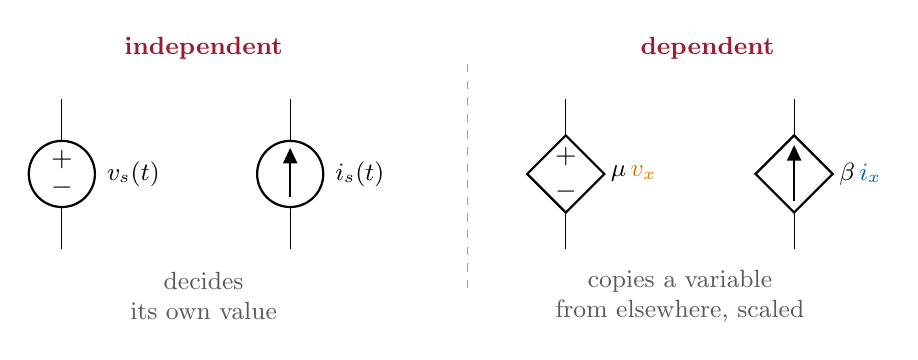
\begin{tikzpicture}[scale=1.0]
    \begin{scope}
      \draw (0,0) to[american voltage source, invert] (0,1.9);
      \node[font=\small, right] at (0.45,0.95) {$v_s(t)$};
    \end{scope}
    \begin{scope}[xshift=2.9cm]
      \draw (0,0) to[american current source] (0,1.9);
      \node[font=\small, right] at (0.45,0.95) {$i_s(t)$};
    \end{scope}
    \draw[metugray!60, dashed] (5.15,-0.5) -- (5.15,2.4);
    \begin{scope}[xshift=6.4cm]
      \draw (0,0) to[american controlled voltage source, invert] (0,1.9);
      \node[font=\small, right] at (0.45,0.95) {$\mu\,\Vcol{v_x}$};
    \end{scope}
    \begin{scope}[xshift=9.3cm]
      \draw (0,0) to[american controlled current source] (0,1.9);
      \node[font=\small, right] at (0.45,0.95) {$\beta\,\Icol{i_x}$};
    \end{scope}
    \node[font=\small\bfseries, text=metured] at (1.8,2.55) {independent};
    \node[font=\small\bfseries, text=metured] at (8.2,2.55) {dependent};
    \node[capn, font=\small] at (1.8,-0.6) {decides\\ its own value};
    \node[capn, font=\small] at (7.85,-0.6) {copies a variable\\ from elsewhere, scaled};
  \end{tikzpicture}
  \end{center}
  \vfill
  \begin{block}{Dependent (controlled) source}
    A voltage or current source whose value is a function of a voltage or current in
    \emph{another} branch --- the \alert{controlling variable}. Almost always the function
    is a constant times one variable: a \alert{linear} dependent source.
  \end{block}
  \vfill
\end{frame}

%--------------------------------------------------------------
\begin{frame}{The four kinds}
  \vfill
  \begin{center}
  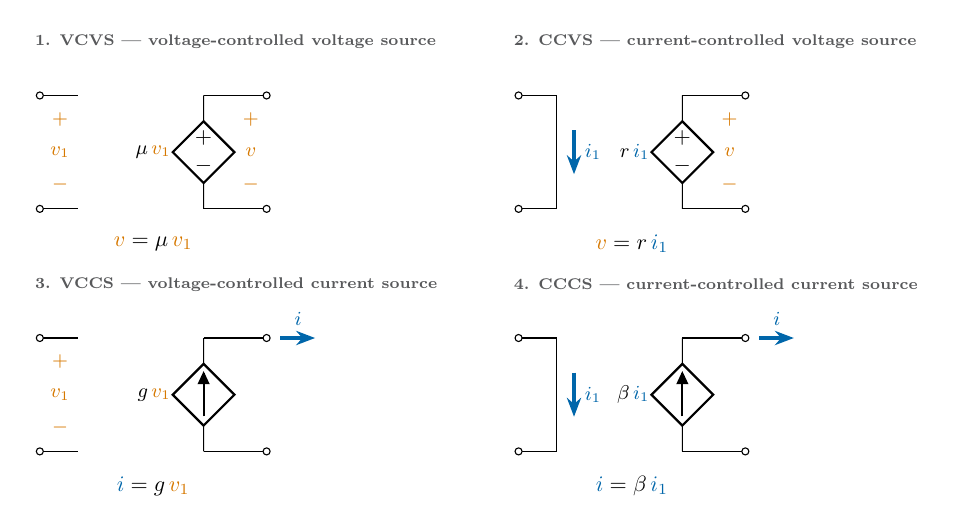
\begin{tikzpicture}[scale=0.8, transform shape]
   \foreach \sx/\sy/\ttlx/\ctl/\out/\val/\eqn in {%
     0/0/{1. VCVS --- voltage-controlled voltage source}/v/v/{$\mu\,\Vcol{v_1}$}/{$\Vcol{v} = \mu\,\Vcol{v_1}$},
     7.6/0/{2. CCVS --- current-controlled voltage source}/i/v/{$r\,\Icol{i_1}$}/{$\Vcol{v} = r\,\Icol{i_1}$},
     0/-3.85/{3. VCCS --- voltage-controlled current source}/v/i/{$g\,\Vcol{v_1}$}/{$\Icol{i} = g\,\Vcol{v_1}$},
     7.6/-3.85/{4. CCCS --- current-controlled current source}/i/i/{$\beta\,\Icol{i_1}$}/{$\Icol{i} = \beta\,\Icol{i_1}$}}{
   \begin{scope}[xshift=\sx cm, yshift=\sy cm]
    \node[ttl, anchor=west] at (-0.2,2.65) {\ttlx};
    \if v\ctl
      \draw (0,0) node[ocirc]{} -- (0.6,0); \draw (0,1.8) node[ocirc]{} -- (0.6,1.8);
      \node[pol] at (0.32,1.42) {$+$}; \node[pol] at (0.32,0.38) {$-$};
      \node[pol] at (0.32,0.9) {$v_1$};
    \else
      \draw (0,0) node[ocirc]{} -- (0.6,0) -- (0.6,1.8) -- (0,1.8) node[ocirc]{};
      \draw[iar] (0.88,1.25) -- (0.88,0.55); \node[font=\small, text=ccur] at (1.18,0.9) {$i_1$};
    \fi
    \if v\out
      \draw (2.6,0) to[american controlled voltage source, invert] (2.6,1.8);
      \node[pol] at (3.35,1.42) {$+$}; \node[pol] at (3.35,0.38) {$-$};
      \node[pol] at (3.35,0.9) {$v$};
    \else
      \draw (2.6,0) to[american controlled current source] (2.6,1.8);
      \draw[iar] (3.82,1.8) -- (4.37,1.8); \node[font=\small, text=ccur] at (4.1,2.1) {$i$};
    \fi
    \draw (2.6,1.8) -- (3.6,1.8) node[ocirc]{}; \draw (2.6,0) -- (3.6,0) node[ocirc]{};
    \node[font=\small, left] at (2.2,0.9) {\val};
    \node[font=\normalsize] at (1.8,-0.55) {\eqn};
   \end{scope}}
  \end{tikzpicture}
  \end{center}
  \vfill
  \begin{center}\small
    The name reads in order: what it \alert{senses}, then what it \alert{produces}.
  \end{center}
\end{frame}

%--------------------------------------------------------------
\begin{frame}{The constant, and its unit}
  \vfill
  \begin{center}\small
  \begin{tabular}{@{}l l l l@{}}
  \toprule
  \textbf{Kind} & \textbf{Equation} & \textbf{The constant} & \textbf{Unit}\\
  \midrule
  VCVS & $\Vcol{v} = \mu\,\Vcol{v_1}$   & voltage gain     & none (V/V)\\
  CCVS & $\Vcol{v} = r\,\Icol{i_1}$     & transresistance  & ohm, $\Omega$ (V/A)\\
  VCCS & $\Icol{i} = g\,\Vcol{v_1}$     & transconductance & siemens, S (A/V)\\
  CCCS & $\Icol{i} = \beta\,\Icol{i_1}$ & current gain     & none (A/A)\\
  \bottomrule
  \end{tabular}
  \end{center}
  \vfill
  \begin{columns}[t,onlytextwidth]
    \begin{column}{0.42\textwidth}
      \small
      The unit is always \alert{what comes out} over \alert{what goes in}.\\[6pt]
      \emph{Trans-} when the two differ: a transresistance turns a current into a voltage,
      so it is measured in ohms.
    \end{column}
    \begin{column}{0.55\textwidth}
      \begin{block}{More general forms}
        \small
        \textbf{Several variables:} $\mu_a\Vcol{v_a} + \mu_b\Vcol{v_b}$ --- one source per
        term.\\[3pt]
        \textbf{Affine:} $\mu\Vcol{v_x} + V_0$ --- plus an independent source $V_0$.\\[3pt]
        \textbf{Nonlinear:} $\Icol{i} = f(\Vcol{v_x})$ --- exists, not used in EE201.
      \end{block}
    \end{column}
  \end{columns}
  \vfill
\end{frame}

%--------------------------------------------------------------
\begin{frame}{The sensing side}
  \vfill
  \begin{columns}[c,onlytextwidth]
    \begin{column}{0.48\textwidth}
      \begin{center}
      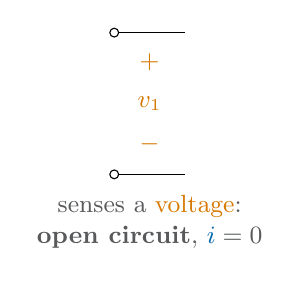
\begin{tikzpicture}[scale=1.0]
        \draw (0,0) node[ocirc]{} -- (0.9,0); \draw (0,1.8) node[ocirc]{} -- (0.9,1.8);
        \node[pol] at (0.45,1.42) {$+$}; \node[pol] at (0.45,0.38) {$-$};
        \node[pol] at (0.45,0.9) {$v_1$};
        \node[capn, font=\small] at (0.45,-0.6) {senses a \Vcol{voltage}:\\ \textbf{open circuit}, $\Icol{i} = 0$};
      \end{tikzpicture}
      \end{center}
    \end{column}
    \begin{column}{0.48\textwidth}
      \begin{center}
      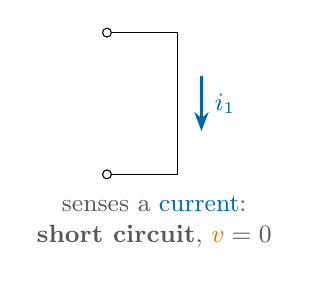
\begin{tikzpicture}[scale=1.0]
        \draw (0,0) node[ocirc]{} -- (0.9,0) -- (0.9,1.8) -- (0,1.8) node[ocirc]{};
        \draw[iar] (1.2,1.25) -- (1.2,0.55); \node[font=\small, text=ccur] at (1.5,0.9) {$i_1$};
        \node[capn, font=\small] at (0.6,-0.6) {senses a \Icol{current}:\\ \textbf{short circuit}, $\Vcol{v} = 0$};
      \end{tikzpicture}
      \end{center}
    \end{column}
  \end{columns}
  \vfill
  \begin{center}
    It senses \alert{without disturbing} anything.\\[6pt]
    In real diagrams this side is \alert{not drawn}: the controlling variable is the voltage
    across,\\ or the current through, an element that is already there --- labelled
    $\Vcol{v_x}$, $\Icol{i_x}$, $\Icol{i_1}$.
  \end{center}
  \vfill
\end{frame}

%--------------------------------------------------------------
\begin{frame}{Why we need them}
  \vfill
  \begin{center}
  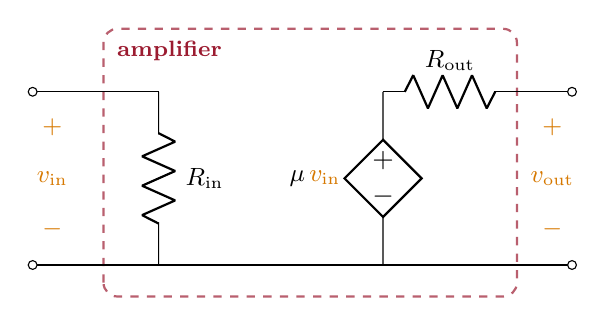
\begin{tikzpicture}[scale=1.0]
    \draw[ampbox] (0.5,-0.4) rectangle (5.75,3.0);
    \node[font=\footnotesize\bfseries, text=metured, anchor=north west] at (0.55,2.97) {amplifier};
    \draw (-0.4,2.2) node[ocirc]{} -- (1.2,2.2);
    \draw (-0.4,0) node[ocirc]{} -- (1.2,0);
    \draw (1.2,0) to[R] (1.2,2.2);
    \node[font=\small, right] at (1.42,1.1) {$R_{\mathrm{in}}$};
    \node[pol] at (-0.15,1.75) {$+$}; \node[pol] at (-0.15,0.45) {$-$};
    \node[pol] at (-0.15,1.1) {$v_{\mathrm{in}}$};
    \draw (4.05,0) to[american controlled voltage source, invert] (4.05,2.2);
    \node[font=\small, left] at (3.63,1.1) {$\mu\,\Vcol{v_{\mathrm{in}}}$};
    \draw (4.05,2.2) to[R] (5.75,2.2) -- (6.45,2.2) node[ocirc]{};
    \node[font=\small] at (4.9,2.6) {$R_{\mathrm{out}}$};
    \draw (1.2,0) -- (6.45,0) node[ocirc]{};
    \node[pol] at (6.2,1.75) {$+$}; \node[pol] at (6.2,0.45) {$-$};
    \node[pol] at (6.2,1.1) {$v_{\mathrm{out}}$};
  \end{tikzpicture}
  \end{center}
  \vfill
  \begin{columns}[c,onlytextwidth]
    \begin{column}{0.38\textwidth}
      \small
      The simplest model of anything that \alert{amplifies}. Many components and
      integrated circuits are modelled as dependent sources --- and some are
      \alert{designed} to be one.
    \end{column}
    \begin{column}{0.60\textwidth}
      \begin{center}\small
      \begin{tabular}{@{}l l l@{}}
      \toprule
      VCVS & op-amp & $\mu \approx 10^5$\\
      CCVS & current-sense amplifier & $r$ \ ($\Omega$)\\
      VCCS & MOSFET, transconductance amp. & $g_m$ \ (S)\\
      CCCS & bipolar transistor & $\beta \approx 100$\\
      \bottomrule
      \end{tabular}
      \end{center}
    \end{column}
  \end{columns}
  \vfill
\end{frame}

%--------------------------------------------------------------
\begin{frame}{Example: what the diamond says}
  \vfill
  \begin{center}
  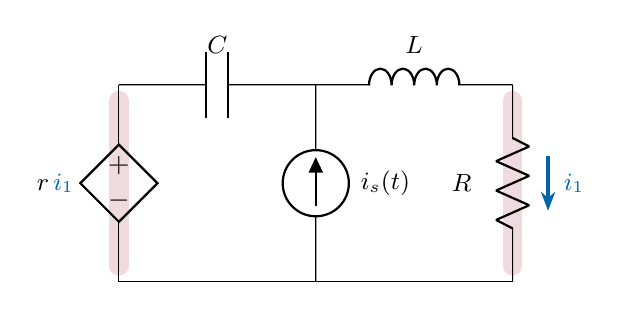
\begin{tikzpicture}[scale=1.0]
    \draw[hal, visible on=<2->] (5.0,2.3) -- (5.0,0.2);
    \draw[hal, visible on=<2->] (0,2.3) -- (0,0.2);
    \draw (0,0) to[american controlled voltage source, invert] (0,2.5);
    \node[font=\small, left] at (-0.45,1.25) {$r\,\Icol{i_1}$};
    \draw (0,2.5) to[C] (2.5,2.5);
    \node[font=\small] at (1.25,3.0) {$C$};
    \draw (2.5,0) to[american current source] (2.5,2.5);
    \node[font=\small, right] at (2.95,1.25) {$i_s(t)$};
    \draw (2.5,2.5) to[L] (5.0,2.5);
    \node[font=\small] at (3.75,3.0) {$L$};
    \draw (5.0,2.5) to[R] (5.0,0);
    \node[font=\small, left] at (4.6,1.25) {$R$};
    \draw[iar] (5.45,1.6) -- (5.45,0.9); \node[font=\small, text=ccur] at (5.78,1.25) {$i_1$};
    \draw (5.0,0) -- (0,0);
  \end{tikzpicture}
  \end{center}
  \vfill
  \begin{center}
    Which equation does the dependent source contribute?\\[8pt]
    \onslide<2->{A CCVS: \ $\Vcol{v} = r\,\Icol{i_1}$ \ --- and $\Icol{i_1}$ flows through
    $R$, at the \alert{far right}.}\\[8pt]
    \onslide<3->{$n = 4$ nodes and $b = 5$ branches: $2b = 10$ unknowns, $b = 5$ terminal
    equations.\\ Four speak about one element each. The fifth \alert{links two branches}.}
  \end{center}
  \vfill
\end{frame}

%--------------------------------------------------------------
\begin{frame}{What is new --- and what is not}
  \vfill
  \begin{center}
  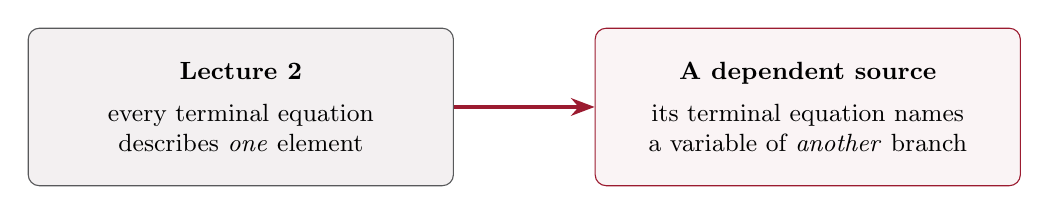
\begin{tikzpicture}[scale=1.0]
    \node[draw=metugray, fill=metulight, rounded corners=4pt, minimum width=5.4cm,
          minimum height=2.0cm, align=center, font=\small] (a) at (0,0)
         {\textbf{Lecture 2}\\[4pt] every terminal equation\\ describes \emph{one} element};
    \node[draw=metured, fill=metured!5, rounded corners=4pt, minimum width=5.4cm,
          minimum height=2.0cm, align=center, font=\small] (b) at (7.2,0)
         {\textbf{A dependent source}\\[4pt] its terminal equation names\\ a variable of
          \emph{another} branch};
    \draw[flowarr] (a) -- (b);
  \end{tikzpicture}
  \end{center}
  \vfill
  \begin{center}
    KCL and KVL are \alert{unchanged}. Still $2b$ equations for $2b$ unknowns.
  \end{center}
  \vfill
  \begin{block}{Two meanings of ``controlled''}
    Lecture 3: a \emph{voltage-controlled resistor} has $\Icol{i} = f(\Vcol{v})$ of its
    \alert{own} voltage. A voltage-controlled \emph{source} takes its value from
    \alert{another} branch.
  \end{block}
  \vfill
\end{frame}

%--------------------------------------------------------------
\begin{frame}{No new method}
  \vfill
  \begin{block}{Recipe}
    \begin{enumerate}\itemsep4pt
      \item Treat the dependent source as if it were independent, with its value written
            as $\mu\Vcol{v_x}$, $r\Icol{i_x}$, $g\Vcol{v_x}$ or $\beta\Icol{i_x}$.
      \item Write KCL, KVL and the terminal equations as usual.
      \item Add one equation that gives the controlling variable in terms of your
            unknowns.
    \end{enumerate}
  \end{block}
  \vfill
  \begin{center}
    The power check $\sum_k \Pcol{p_k} = 0$ still works --- \alert{include} the dependent
    source.
  \end{center}
  \vfill
\end{frame}

%--------------------------------------------------------------
\begin{frame}{Example: an amplifier}
  \begin{center}
  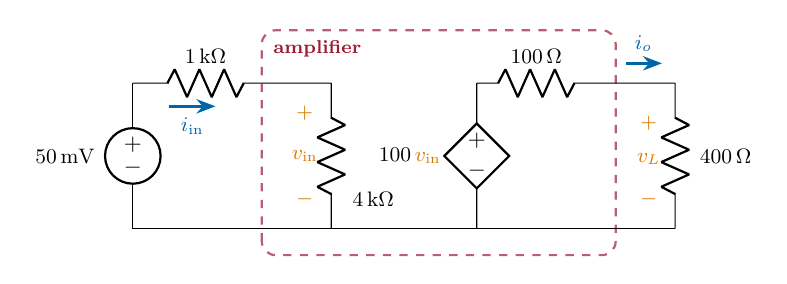
\begin{tikzpicture}[scale=0.84, transform shape]
    \draw[ampbox] (1.95,-0.4) rectangle (7.3,3.0);
    \node[font=\footnotesize\bfseries, text=metured, anchor=north west] at (2.0,2.97) {amplifier};
    \draw (0,0) to[american voltage source, invert] (0,2.2);
    \node[font=\small, left] at (-0.45,1.1) {$50\uni{mV}$};
    \draw (0,2.2) to[R] (2.2,2.2) -- (3.0,2.2);
    \node[font=\small] at (1.1,2.6) {$1\kohm$};
    \draw[iar] (0.55,1.85) -- (1.25,1.85); \node[font=\small, text=ccur] at (0.9,1.55) {$i_{\mathrm{in}}$};
    \draw (3.0,0) to[R] (3.0,2.2);
    \node[font=\small, anchor=west] at (3.2,0.45) {$4\kohm$};
    \node[pol] at (2.6,1.75) {$+$}; \node[pol] at (2.6,1.1) {$v_{\mathrm{in}}$};
    \node[pol] at (2.6,0.45) {$-$};
    \draw (5.2,0) to[american controlled voltage source, invert] (5.2,2.2);
    \node[font=\small, left] at (4.78,1.1) {$100\,\Vcol{v_{\mathrm{in}}}$};
    \draw (5.2,2.2) to[R] (7.0,2.2) -- (8.2,2.2);
    \node[font=\small] at (6.1,2.6) {$100\ohm$};
    \draw[iar] (7.45,2.5) -- (8.0,2.5); \node[font=\small, text=ccur] at (7.72,2.8) {$i_o$};
    \draw (8.2,2.2) to[R] (8.2,0);
    \node[font=\small, anchor=west] at (8.45,1.1) {$400\ohm$};
    \node[pol] at (7.8,1.6) {$+$}; \node[pol] at (7.8,1.05) {$v_L$}; \node[pol] at (7.8,0.45) {$-$};
    \draw (8.2,0) -- (0,0);
  \end{tikzpicture}
  \end{center}
  \vspace{-2pt}
  \begin{center}\small
    A microphone drives an amplifier with $\mu = 100$. \ Find $\Vcol{v_L}$.
  \end{center}
  \vspace{-4pt}
  \begin{columns}[t,onlytextwidth]
    \begin{column}{0.48\textwidth}
      \onslide<2->
      \textbf{Input side} --- a divider:
      \[ \Icol{i_{\mathrm{in}}} = \frac{50\uni{mV}}{5\kohm} = 10\uni{\mu A} \]
      \[ \Vcol{v_{\mathrm{in}}} = 4\kohm \times 10\uni{\mu A} = 40\uni{mV} \]
    \end{column}
    \begin{column}{0.48\textwidth}
      \onslide<3->
      \textbf{Output side} --- the diamond is $4\V$:
      \[ \Icol{i_o} = \frac{4\V}{500\ohm} = 8\uni{mA} \]
      \[ \alert{\Vcol{v_L} = 3.2\V}, \qquad \frac{\Vcol{v_L}}{v_s} = 64 \]
    \end{column}
  \end{columns}
\end{frame}

%--------------------------------------------------------------
\begin{frame}{Where the power comes from}
  \vfill
  \begin{columns}[c,onlytextwidth]
    \begin{column}{0.46\textwidth}
      \begin{center}
      \begin{tabular}{@{}l r@{}}
      \toprule
      \textbf{input side} & \\
      \midrule
      microphone & $-0.5\uni{\mu W}$\\
      $R_s$      & $+0.1\uni{\mu W}$\\
      $R_{\mathrm{in}}$ & $+0.4\uni{\mu W}$\\
      \bottomrule
      \end{tabular}
      \end{center}
    \end{column}
    \begin{column}{0.50\textwidth}
      \onslide<2->
      \begin{center}
      \begin{tabular}{@{}l r@{}}
      \toprule
      \textbf{output side} & \\
      \midrule
      dependent source & $-32\uni{mW}$\\
      $R_{\mathrm{out}}$ & $+6.4\uni{mW}$\\
      $R_L$            & $+25.6\uni{mW}$\\
      \bottomrule
      \end{tabular}
      \end{center}
    \end{column}
  \end{columns}
  \vfill
  \begin{center}
    \onslide<2->{Each side sums to zero.}\\[6pt]
    \onslide<3->{The load gets \alert{$51\,200$ times} what the microphone supplies.\\
    The \alert{dependent source} delivered it. A real amplifier takes it from its power
    supply,\\ which the model does not draw.}
  \end{center}
  \vfill
\end{frame}

%--------------------------------------------------------------
\begin{frame}{The shared wire carries no current}
  \vfill
  \begin{center}
  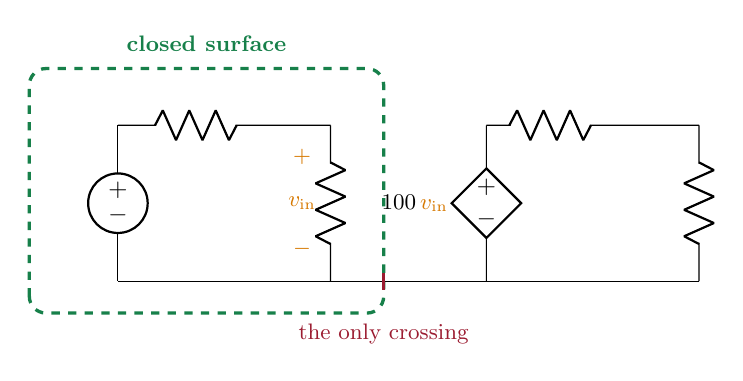
\begin{tikzpicture}[scale=0.9, transform shape]
    \draw[surf] (-1.25,-0.45) rectangle (3.75,3.0);
    \node[font=\small\bfseries, text=cpow] at (1.25,3.35) {closed surface};
    \draw (0,0) to[american voltage source, invert] (0,2.2);
    \draw (0,2.2) to[R] (2.2,2.2) -- (3.0,2.2);
    \draw (3.0,0) to[R] (3.0,2.2);
    \node[pol] at (2.6,1.75) {$+$}; \node[pol] at (2.6,1.1) {$v_{\mathrm{in}}$};
    \node[pol] at (2.6,0.45) {$-$};
    \draw (5.2,0) to[american controlled voltage source, invert] (5.2,2.2);
    \node[font=\small, left] at (4.78,1.1) {$100\,\Vcol{v_{\mathrm{in}}}$};
    \draw (5.2,2.2) to[R] (7.0,2.2) -- (8.2,2.2);
    \draw (8.2,2.2) to[R] (8.2,0);
    \draw (8.2,0) -- (0,0);
    \draw[metured, very thick] (3.75,-0.12) -- (3.75,0.12);
    \node[font=\small, text=metured] at (3.75,-0.75) {the only crossing};
  \end{tikzpicture}
  \end{center}
  \vfill
  \begin{center}
    KCL on the surface (Lecture 2): one branch crosses it, so its current is \alert{zero}.\\[6pt]
    The two sides interact \alert{only} through $\Vcol{v_{\mathrm{in}}}$.
  \end{center}
  \vfill
\end{frame}

%--------------------------------------------------------------
\begin{frame}{Example: when the controlling variable is unknown}
  \begin{columns}[c,onlytextwidth]
    \begin{column}{0.47\textwidth}
      \begin{center}
      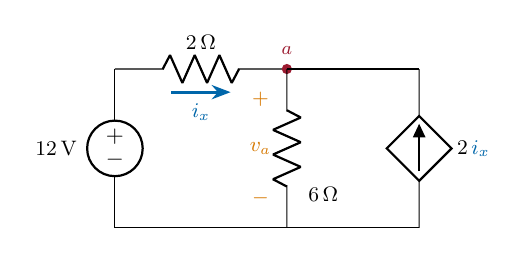
\begin{tikzpicture}[scale=0.84, transform shape]
        \draw (0,0) to[american voltage source, invert] (0,2.4);
        \node[font=\small, left] at (-0.45,1.2) {$12\V$};
        \draw (0,2.4) to[R] (2.6,2.4);
        \node[font=\small] at (1.3,2.8) {$2\ohm$};
        \draw[iar] (0.85,2.05) -- (1.75,2.05); \node[font=\small, text=ccur] at (1.3,1.75) {$i_x$};
        \fill[metured] (2.6,2.4) circle (2.2pt); \node[glab, above] at (2.6,2.5) {$a$};
        \draw (2.6,0) to[R] (2.6,2.4);
        \node[font=\small, right] at (2.8,0.5) {$6\ohm$};
        \node[pol] at (2.2,1.95) {$+$}; \node[pol] at (2.2,1.2) {$v_a$}; \node[pol] at (2.2,0.45) {$-$};
        \draw (2.6,2.4) -- (4.6,2.4);
        \draw (4.6,0) to[american controlled current source] (4.6,2.4);
        \node[font=\small, right] at (5.05,1.2) {$2\,\Icol{i_x}$};
        \draw (4.6,0) -- (0,0);
      \end{tikzpicture}
      \end{center}
      \begin{center}\small Find $\Icol{i_x}$ and $\Vcol{v_a}$.\end{center}
    \end{column}
    \begin{column}{0.51\textwidth}
      \small
      \onslide<2->
      \textbf{Equations} --- $\Icol{i_x}$ is already an unknown:
      \[ \text{KVL: } -12 + 2\Icol{i_x} + \Vcol{v_a} = 0 \]
      \[ \text{KCL at } a\text{: } -\Icol{i_x} - 2\Icol{i_x} + \tfrac{\Vcol{v_a}}{6} = 0
         \;\Rightarrow\; \Vcol{v_a} = 18\,\Icol{i_x} \]
      \onslide<3->
      \textbf{Solution:} $-12 + 20\,\Icol{i_x} = 0$
      \[ \alert{\Icol{i_x} = 0.6\A}, \qquad \alert{\Vcol{v_a} = 10.8\V} \]
      \onslide<4->
      \textbf{Power check:}
      \[ \underbrace{-7.2}_{12\V} + \underbrace{0.72}_{2\Omega} + \underbrace{19.44}_{6\Omega}
         \underbrace{-\,12.96}_{\text{CCCS}} = 0 \]
      The CCCS carries $1.2\A$ \emph{out of} its $+$ terminal: it \alert{delivers}.
    \end{column}
  \end{columns}
\end{frame}

%--------------------------------------------------------------
\begin{frame}{What a dependent source cannot do}
  \vfill
  \begin{block}{It cannot start anything}
    Switch the $12\V$ off: $2\Icol{i_x} + \Vcol{v_a} = 0$ and $\Vcol{v_a} = 18\Icol{i_x}$,
    so $20\,\Icol{i_x} = 0$.\\ Every voltage and current is zero --- the dependent source's
    too.
  \end{block}
  \vfill
  \begin{block}{It is never switched off}
    Later we switch sources off one at a time (superposition, Thévenin). Only
    \alert{independent} sources are switched off: a dependent source is part of how the
    circuit behaves, not an input.
  \end{block}
  \vfill
\end{frame}

%==============================================================
\begin{frame}{Two coils, one core}
  \vfill
  \begin{columns}[c,onlytextwidth]
    \begin{column}{0.56\textwidth}
      \begin{center}
      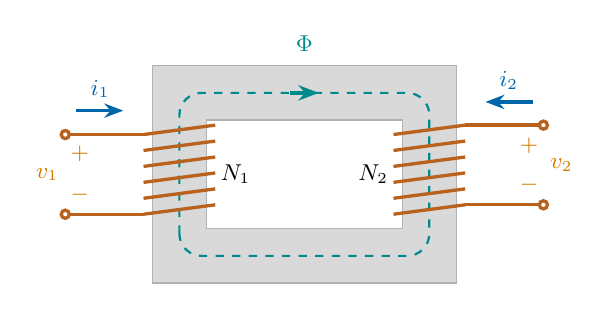
\begin{tikzpicture}[scale=0.92, transform shape]
        \fill[gray!30, even odd rule] (0,0) rectangle (4.2,3.0) (0.75,0.75) rectangle (3.45,2.25);
        \draw[gray!60] (0,0) rectangle (4.2,3.0); \draw[gray!60] (0.75,0.75) rectangle (3.45,2.25);
        \draw[cflux, thick, dashed, rounded corners=8pt] (0.375,0.375) rectangle (3.825,2.625);
        \draw[-{Stealth[length=2.6mm]}, cflux, very thick] (1.9,2.625) -- (2.3,2.625);
        \node[font=\small, text=cflux] at (2.1,3.3) {$\Fcol{\Phi}$};
        \foreach \y in {0.95,1.17,...,2.05}{
          \draw[copper, very thick] (-0.12,\y) -- (0.87,\y+0.13);
          \draw[copper, very thick] (3.33,\y) -- (4.32,\y+0.13);}
        \draw[copper, very thick] (-0.12,2.05) -- (-1.2,2.05) node[ocirc]{};
        \draw[copper, very thick] (-0.12,0.95) -- (-1.2,0.95) node[ocirc]{};
        \draw[copper, very thick] (4.32,2.18) -- (5.4,2.18) node[ocirc]{};
        \draw[copper, very thick] (4.32,1.08) -- (5.4,1.08) node[ocirc]{};
        \node[font=\small] at (1.15,1.5) {$N_1$};  \node[font=\small] at (3.05,1.5) {$N_2$};
        \node[pol] at (-1.0,1.78) {$+$}; \node[pol] at (-1.0,1.22) {$-$};
        \node[pol] at (-1.45,1.5) {$v_1$};
        \node[pol] at (5.2,1.9) {$+$}; \node[pol] at (5.2,1.36) {$-$};
        \node[pol] at (5.65,1.63) {$v_2$};
        \draw[iar] (-1.05,2.38) -- (-0.4,2.38); \node[font=\small, text=ccur] at (-0.72,2.68) {$i_1$};
        \draw[iar] (5.25,2.5) -- (4.6,2.5); \node[font=\small, text=ccur] at (4.92,2.8) {$i_2$};
      \end{tikzpicture}
      \end{center}
    \end{column}
    \begin{column}{0.42\textwidth}
      \small
      \begin{itemize}\itemsep5pt
        \item \textbf{Lecture 1:} no changing magnetic field links the loops.
        \item \textbf{Lecture 2:} if we \emph{want} such a link, draw it as an element.
        \item \textbf{Lecture 5:} a coil's field passes through the coil itself.
        \item \textbf{Today:} two coils on one iron core --- the field of each passes
              through the other.
      \end{itemize}
    \end{column}
  \end{columns}
  \vfill
\end{frame}

%--------------------------------------------------------------
\begin{frame}{The ideal transformer}
  \vfill
  \begin{columns}[c,onlytextwidth]
    \begin{column}{0.42\textwidth}
      \begin{center}
      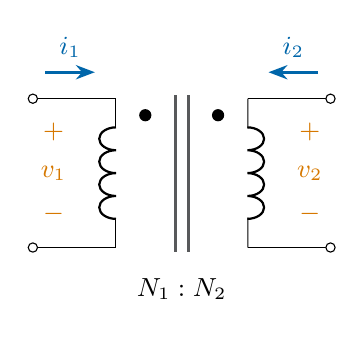
\begin{tikzpicture}[scale=1.05, transform shape]
        \xfmr{0}{1.8}
        \draw (0,1.8) -- (-1.0,1.8) node[ocirc]{};  \draw (0,0) -- (-1.0,0) node[ocirc]{};
        \draw (1.6,1.8) -- (2.6,1.8) node[ocirc]{}; \draw (1.6,0) -- (2.6,0) node[ocirc]{};
        \node[pol] at (-0.75,1.4) {$+$}; \node[pol] at (-0.75,0.4) {$-$};
        \node[pol] at (-0.75,0.9) {$v_1$};
        \node[pol] at (2.35,1.4) {$+$}; \node[pol] at (2.35,0.4) {$-$};
        \node[pol] at (2.35,0.9) {$v_2$};
        \draw[iar] (-0.85,2.12) -- (-0.25,2.12); \node[font=\small, text=ccur] at (-0.55,2.42) {$i_1$};
        \draw[iar] (2.45,2.12) -- (1.85,2.12); \node[font=\small, text=ccur] at (2.15,2.42) {$i_2$};
        \node[font=\small] at (0.8,-0.5) {$N_1 : N_2$};
      \end{tikzpicture}
      \end{center}
    \end{column}
    \begin{column}{0.56\textwidth}
      \begin{block}{Two equations}
        \[ \frac{\Vcol{v_1}}{N_1} = \frac{\Vcol{v_2}}{N_2}
           \qquad\qquad N_1\Icol{i_1} + N_2\Icol{i_2} = 0 \]
        $\Vcol{v}$ positive and $\Icol{i}$ entering at the \alert{dots}.
      \end{block}
      \vspace{4pt}
      \small
      Equivalently $\Vcol{v_2} = \tfrac{N_2}{N_1}\Vcol{v_1}$, \
      $\Icol{i_2} = -\tfrac{N_1}{N_2}\Icol{i_1}$.\\[6pt]
      The dots act like reference marks. Move one dot and both equations
      \alert{change sign}.
    \end{column}
  \end{columns}
  \vfill
\end{frame}

%--------------------------------------------------------------
\begin{frame}{Where the two equations come from}
  \vfill
  \begin{block}{Voltages: one flux through every turn}
    Each turn sees $d\Fcol{\Phi}/dt$. $N$ turns in series: $\Vcol{v} = N\,d\Fcol{\Phi}/dt$.
    \[ \frac{\Vcol{v_1}}{N_1} = \frac{\Vcol{v_2}}{N_2} = \frac{d\Fcol{\Phi}}{dt} \]
  \end{block}
  \vfill
  \begin{block}{Currents: an ideal core needs no current}
    The turn-weighted currents must cancel: \ $N_1\Icol{i_1} + N_2\Icol{i_2} = 0$.\\
    A real core needs a small magnetising current; the ideal one needs none.
  \end{block}
  \vfill
  \begin{center}\small
    With $k$ windings on one core: \
    $\dfrac{\Vcol{v_1}}{N_1} = \cdots = \dfrac{\Vcol{v_k}}{N_k}$ \ and \
    $N_1\Icol{i_1} + \cdots + N_k\Icol{i_k} = 0$.
  \end{center}
  \vfill
\end{frame}

%--------------------------------------------------------------
\begin{frame}{No derivatives --- and no DC}
  \vfill
  \begin{center}
    {\large The equations are \alert{algebraic}: no $d/dt$, no memory.}\\[6pt]
    The ideal transformer is a \alert{resistive} element --- listed with resistors and\\
    dependent sources in the course outline, even though it is built from coils.
  \end{center}
  \vfill
  \begin{block}{A real transformer needs a changing flux}
    Feed it DC and, once the current settles, the flux is constant: the secondary voltage
    is zero and the primary is just a coil --- a \alert{short circuit} at DC (Lecture 5).
    Use the ideal model for changing waveforms only.
  \end{block}
  \vfill
\end{frame}

%--------------------------------------------------------------
\begin{frame}{The ideal transformer absorbs no power}
  \vfill
  \begin{center}
    Each winding obeys the PSC, so $\Vcol{v_j}\Icol{i_j}$ is what it absorbs.\\[8pt]
    {\Large $\displaystyle \Pcol{p(t)} = \sum_{j=1}^{k} \Vcol{v_j}\Icol{i_j} = 0$
     \quad \normalsize at every instant}
  \end{center}
  \vfill
  \begin{center}
    \onslide<2->{Call the common ratio $\lambda(t) = \Vcol{v_j}/N_j$, so
    $\Vcol{v_j} = N_j\lambda$:}\\[6pt]
    \onslide<3->{\[ \sum_j \Vcol{v_j}\Icol{i_j} = \sum_j N_j\lambda\,\Icol{i_j}
       = \lambda \underbrace{\sum_j N_j\Icol{i_j}}_{=\,0} = 0 \]}
    \onslide<4->{The first equation gave $\lambda$; the second made the sum vanish.
    \alert{Both} are needed.}
  \end{center}
  \vfill
\end{frame}

%--------------------------------------------------------------
\begin{frame}{Dissipate, store, or pass through}
  \vfill
  \begin{center}
  \begin{tabular}{@{}l l l@{}}
  \toprule
  \textbf{Element} & \textbf{Absorbed power} & \textbf{The energy is}\\
  \midrule
  resistor            & $\Pcol{p} \ge 0$               & dissipated\\
  capacitor, inductor & $\Pcol{p}$ can change sign     & stored, then returned\\
  ideal transformer   & $\Pcol{p} = 0$ at every instant & passed straight through\\
  \bottomrule
  \end{tabular}
  \end{center}
  \vfill
  \begin{center}
    Two windings: \ $\Vcol{v_1}\Icol{i_1} = -\Vcol{v_2}\Icol{i_2}$.\\[6pt]
    Voltage multiplied by $N_2/N_1$, current divided by $N_2/N_1$ --- the
    \alert{product unchanged}.
  \end{center}
  \vfill
\end{frame}

%--------------------------------------------------------------
\begin{frame}{Example: a step-down transformer}
  \begin{center}
  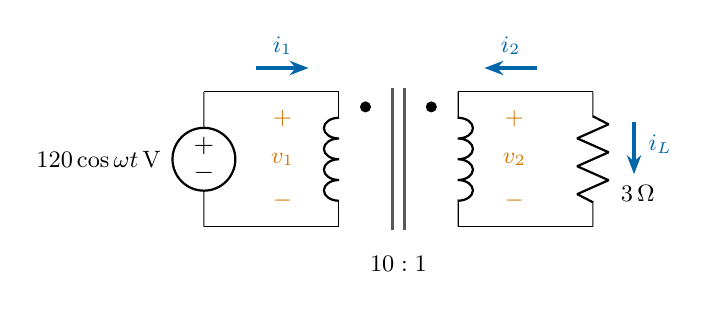
\begin{tikzpicture}[scale=0.95, transform shape]
    \draw (-1.8,0) to[american voltage source, invert] (-1.8,1.8);
    \node[font=\small, left] at (-2.25,0.9) {$120\cos\omega t\V$};
    \draw (-1.8,1.8) -- (0,1.8); \draw (-1.8,0) -- (0,0);
    \xfmr{0}{1.8}
    \draw (1.6,1.8) -- (3.4,1.8); \draw (1.6,0) -- (3.4,0);
    \draw (3.4,1.8) to[R] (3.4,0);
    \node[font=\small, right] at (3.65,0.45) {$3\ohm$};
    \draw[iar] (3.95,1.4) -- (3.95,0.7); \node[font=\small, text=ccur] at (4.3,1.1) {$i_L$};
    \node[pol] at (-0.75,1.45) {$+$}; \node[pol] at (-0.75,0.9) {$v_1$}; \node[pol] at (-0.75,0.35) {$-$};
    \node[pol] at (2.35,1.45) {$+$}; \node[pol] at (2.35,0.9) {$v_2$}; \node[pol] at (2.35,0.35) {$-$};
    \draw[iar] (-1.1,2.12) -- (-0.4,2.12); \node[font=\small, text=ccur] at (-0.75,2.42) {$i_1$};
    \draw[iar] (2.65,2.12) -- (1.95,2.12); \node[font=\small, text=ccur] at (2.3,2.42) {$i_2$};
    \node[font=\small] at (0.8,-0.5) {$10 : 1$};
  \end{tikzpicture}
  \end{center}
  \begin{center}\small Find the currents and the power on each side.\end{center}
  \vspace{-4pt}
  \begin{columns}[t,onlytextwidth]
    \begin{column}{0.5\textwidth}
      \small
      \onslide<2->
      $\Vcol{v_2} = \tfrac{1}{10}\Vcol{v_1} = 12\cos\omega t\V$\\[3pt]
      $\Icol{i_L} = \Vcol{v_2}/3 = 4\cos\omega t\A$, \ so
      $\Icol{i_2} = -4\cos\omega t\A$\\[3pt]
      $\Icol{i_1} = -\tfrac{1}{10}\Icol{i_2} = 0.4\cos\omega t\A$
    \end{column}
    \begin{column}{0.48\textwidth}
      \small
      \onslide<3->
      $\Pcol{p_1} = \Vcol{v_1}\Icol{i_1} = 48\cos^2\omega t\W$\\[3pt]
      $\Pcol{p_2} = \Vcol{v_2}\Icol{i_2} = -48\cos^2\omega t\W$\\[3pt]
      $\Pcol{p_1} + \Pcol{p_2} = 0$ --- \alert{at every instant}.
    \end{column}
  \end{columns}
\end{frame}

%--------------------------------------------------------------
\begin{frame}{Seen from the source}
  \vfill
  \begin{center}
    $\dfrac{\Vcol{v_1}}{\Icol{i_1}} = \dfrac{120}{0.4} = 300\ohm = 10^2 \times 3\ohm$\\[10pt]
    The source cannot tell the transformer and its $3\ohm$ load from a single $300\ohm$
    resistor.
  \end{center}
  \vfill
  \begin{block}{A transformer rescales resistance}
    \[ \frac{\Vcol{v_1}}{\Icol{i_1}} = \Bigl(\frac{N_1}{N_2}\Bigr)^{\!2} R_L \]
    That is how an $8\ohm$ loudspeaker is made to look like a much larger resistance to
    the amplifier driving it.
  \end{block}
  \vfill
\end{frame}

%--------------------------------------------------------------
\begin{frame}{A transformer is two dependent sources}
  \vfill
  \begin{center}
  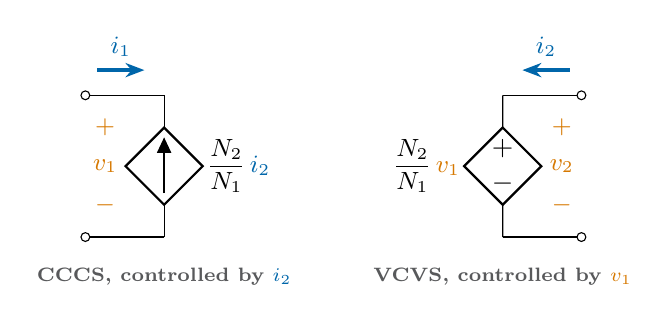
\begin{tikzpicture}[scale=1.0]
    \draw (0,0) to[american controlled current source] (0,1.8);
    \node[font=\small, right] at (0.42,0.9) {$\dfrac{N_2}{N_1}\,\Icol{i_2}$};
    \draw (0,1.8) -- (-1.0,1.8) node[ocirc]{}; \draw (0,0) -- (-1.0,0) node[ocirc]{};
    \node[pol] at (-0.75,1.4) {$+$}; \node[pol] at (-0.75,0.4) {$-$};
    \node[pol] at (-0.75,0.9) {$v_1$};
    \draw[iar] (-0.85,2.12) -- (-0.25,2.12); \node[font=\small, text=ccur] at (-0.55,2.42) {$i_1$};
    \draw (4.3,0) to[american controlled voltage source, invert] (4.3,1.8);
    \node[font=\small, left] at (3.88,0.9) {$\dfrac{N_2}{N_1}\,\Vcol{v_1}$};
    \draw (4.3,1.8) -- (5.3,1.8) node[ocirc]{}; \draw (4.3,0) -- (5.3,0) node[ocirc]{};
    \node[pol] at (5.05,1.4) {$+$}; \node[pol] at (5.05,0.4) {$-$};
    \node[pol] at (5.05,0.9) {$v_2$};
    \draw[iar] (5.15,2.12) -- (4.55,2.12); \node[font=\small, text=ccur] at (4.85,2.42) {$i_2$};
    \node[ttl] at (0,-0.5) {CCCS, controlled by $\Icol{i_2}$};
    \node[ttl] at (4.3,-0.5) {VCVS, controlled by $\Vcol{v_1}$};
  \end{tikzpicture}
  \end{center}
  \vfill
  \begin{center}
    \onslide<2->{CCCS: $\Icol{i_1} = -\tfrac{N_2}{N_1}\Icol{i_2}$ \ is \
    $N_1\Icol{i_1} + N_2\Icol{i_2} = 0$. \qquad
    VCVS: $\Vcol{v_2} = \tfrac{N_2}{N_1}\Vcol{v_1}$.}\\[8pt]
    \onslide<3->{Powers: $-\tfrac{N_2}{N_1}\Vcol{v_1}\Icol{i_2}$ and
    $+\tfrac{N_2}{N_1}\Vcol{v_1}\Icol{i_2}$ --- one delivers exactly what the other
    absorbs.}
  \end{center}
  \vfill
\end{frame}

%--------------------------------------------------------------
\begin{frame}{Summary}
  \vfill
  \begin{itemize}\itemsep5pt
    \item A \textbf{dependent source} (diamond) takes its value from a voltage or current in
          another branch: VCVS, CCVS, VCCS, CCCS. Unit of the constant: out over in.
          Almost always linear in one variable.
    \item Its terminal equation names a \alert{foreign variable}. Write KCL, KVL and
          terminal equations as usual, plus one equation for the controlling variable.
    \item It can \textbf{deliver power} --- that is amplification --- but it
          \textbf{cannot start anything}, and it is never switched off.
    \item \textbf{Ideal transformer}: $\Vcol{v_1}/N_1 = \Vcol{v_2}/N_2$, \
          $N_1\Icol{i_1} + N_2\Icol{i_2} = 0$, signs set by the \alert{dots}. Resistive, but a
          real one needs changing waveforms.
    \item It \textbf{absorbs no power at any instant} and rescales a load by
          $(N_1/N_2)^2$.
  \end{itemize}
  \vfill
\end{frame}

%--------------------------------------------------------------
\begin{frame}{Next lecture}
  \vfill
  \begin{center}
  \begin{block}{From circuit to graph}
    Labelling the nodes and branches of a circuit so that its $2b$ equations can be
    written systematically --- the first step towards node and mesh analysis.
  \end{block}
  \end{center}
  \vfill
  \begin{center}
    {\Large\color{metured} Questions?}
  \end{center}
  \vfill
\end{frame}

\end{document}
